\begin{frame}[plain]
	\frametitle{Existence Theory}
	\begin{textblock*}{70mm}(30mm,25mm)
		\begin{greenbox}{}
			$$\left\{ \begin{array}{l}
			\dot{x}(s)=f(s,u(s),x(s))\,\,s\in [t_0,T], \\
			x(t_0)=x_0,\\
			\end{array}
			\right.$$
	
			with terminal state constraint
			$$x(T;t_0,x_0,u(\cdot))\in M, M\subseteq \mathbb{R}^n.$$
			
		\end{greenbox}
	\end{textblock*}
	\begin{textblock*}{100mm}(15mm,65mm)
		\begin{yellowbox}{}
			$$J(t_0,x_0;u(\cdot))=\int_{t_0}^{T}g(s,u(s),x(s))ds+h(x(T)).$$
		\end{yellowbox}
	\end{textblock*}
\end{frame}
%%%%%%%%%%%%%%%%%%%%%%%%%%%%%%%%%%%%%%%%%%%%%%%%%%%%%%%%%%%%%%%%%%%%%%%%%%%%%%%%

\begin{frame}[plain]
	\begin{textblock*}{110mm}(10mm,20mm)
		\begin{graybox}{Problem $(OC)$}
			$(t_0,x_0)\in \mathbb{R}_{+}\times \mathbb{R}^n$ with $\mathcal{U}_{x_0}[t_0,T]\neq\emptyset$, find a $\bar{u}(\cdot)\in \mathcal{U}_{x_0}[t_0,T]$ s.t.
			
			\begin{equation*}
				J(t_0,x_0;\bar{u}(\cdot))=\inf_{u(\cdot)\in \mathcal{U}_{x_0}[t_0,T]} J(t_0,x_0;u(\cdot)).
			\end{equation*}
		\end{graybox}
	\end{textblock*}
\end{frame}
%%%%%%%%%%%%%%%%%%%%%%%%%%%%%%%%%%%%%%%%%%%%%%%%%%%%%%%%%%%%%%%%%%%%%%%%%%%%%%%%
\begin{frame}[plain]
	\only<1,2,3,5>{
	\begin{textblock*}{60mm}(5mm,5mm)
		\begin{graybox}{Hypothesis:}
			\begin{enumerate}[(\textbf{{C}}-1)]
				\item<1->
					$
						f:\mathbb{R}_{+}\times U
						\times \mathbb{R}^n\rightarrow 
						\mathbb{R}^n
					$ is measurable, satisfies a lipchitz
					 condition in $x$,
					$
						|f(t,u,0)|\leq L,\,
						 \forall\,(t,u)\in
						 \mathbb{R}_{+}\times U .
					$
				\item<2->
					$
						g:\mathbb{R}_{+}\times U\times 
						\mathbb{R}^n\rightarrow \mathbb{R},
					$ 
					$
						h:\mathbb{R}^n\rightarrow \mathbb{R}
					$ are measurable, and
					\begin{align*}
						&|g(s,u,x_1)-g(s,u,x_2)|+\\
						&|h(x_1)-h(x_2)|\\
						&\leq \omega(|x_1|\vee |x_2|,|x_1-x_2|)
					\end{align*}
					$
						\forall\, (s,u)\in \mathbb{R}_{+}
						\times U,x_1,x_2\in \mathbb{R}^n
					$.
				\item<3->
					For a.a. $t\in[0,T]$, Cesari property holds $\forall$ $x\in \mathbb{R}^n$.
			\end{enumerate}	
		\end{graybox}
	\end{textblock*}
	}
	\only<2>
	{
		\begin{textblock*}{50mm}(75mm,5mm)
			\begin{yellowbox}{Modulus of continuity}
				$\omega:\mathbb{R}_{+}\times\mathbb{R}_{+}\rightarrow \mathbb{R}_{+}$, increasing, $\omega(r,0)=0$ 
				${\forall r\geq 0}$.
			\end{yellowbox}
		\end{textblock*}
	}
	\only<3,4>
	{
		\begin{textblock*}{50mm}(75mm,20mm)
			\begin{yellowbox}{}
				$\bar{co}(\mathbf{E})$: closed convex hull of $\mathbf{E}$,
				\begin{align*}
					&\mathbf{E}(t,x)=\{(z^0,z)\in \mathbb{R}\times \mathbb{R}^n|\\
					&z^0\geq g(t,u,x),\\
					&z=f(t,u,x),\, u\in U\}.
				\end{align*}			
			\end{yellowbox}
		\end{textblock*}
	
		\begin{textblock*}{50mm}(75mm,60mm)
			\begin{yellowbox}{Cesari property}
				\begin{equation*}
				\bigcap_{\delta>0}\bar{co}\mathbf{E}(t,B_{\delta}(x))=\mathbf{E}(t,x)
				\end{equation*}			
			\end{yellowbox}
		\end{textblock*}
	}
	\only<4>
	{
		\begin{textblock*}{60mm}(5mm,30mm)
			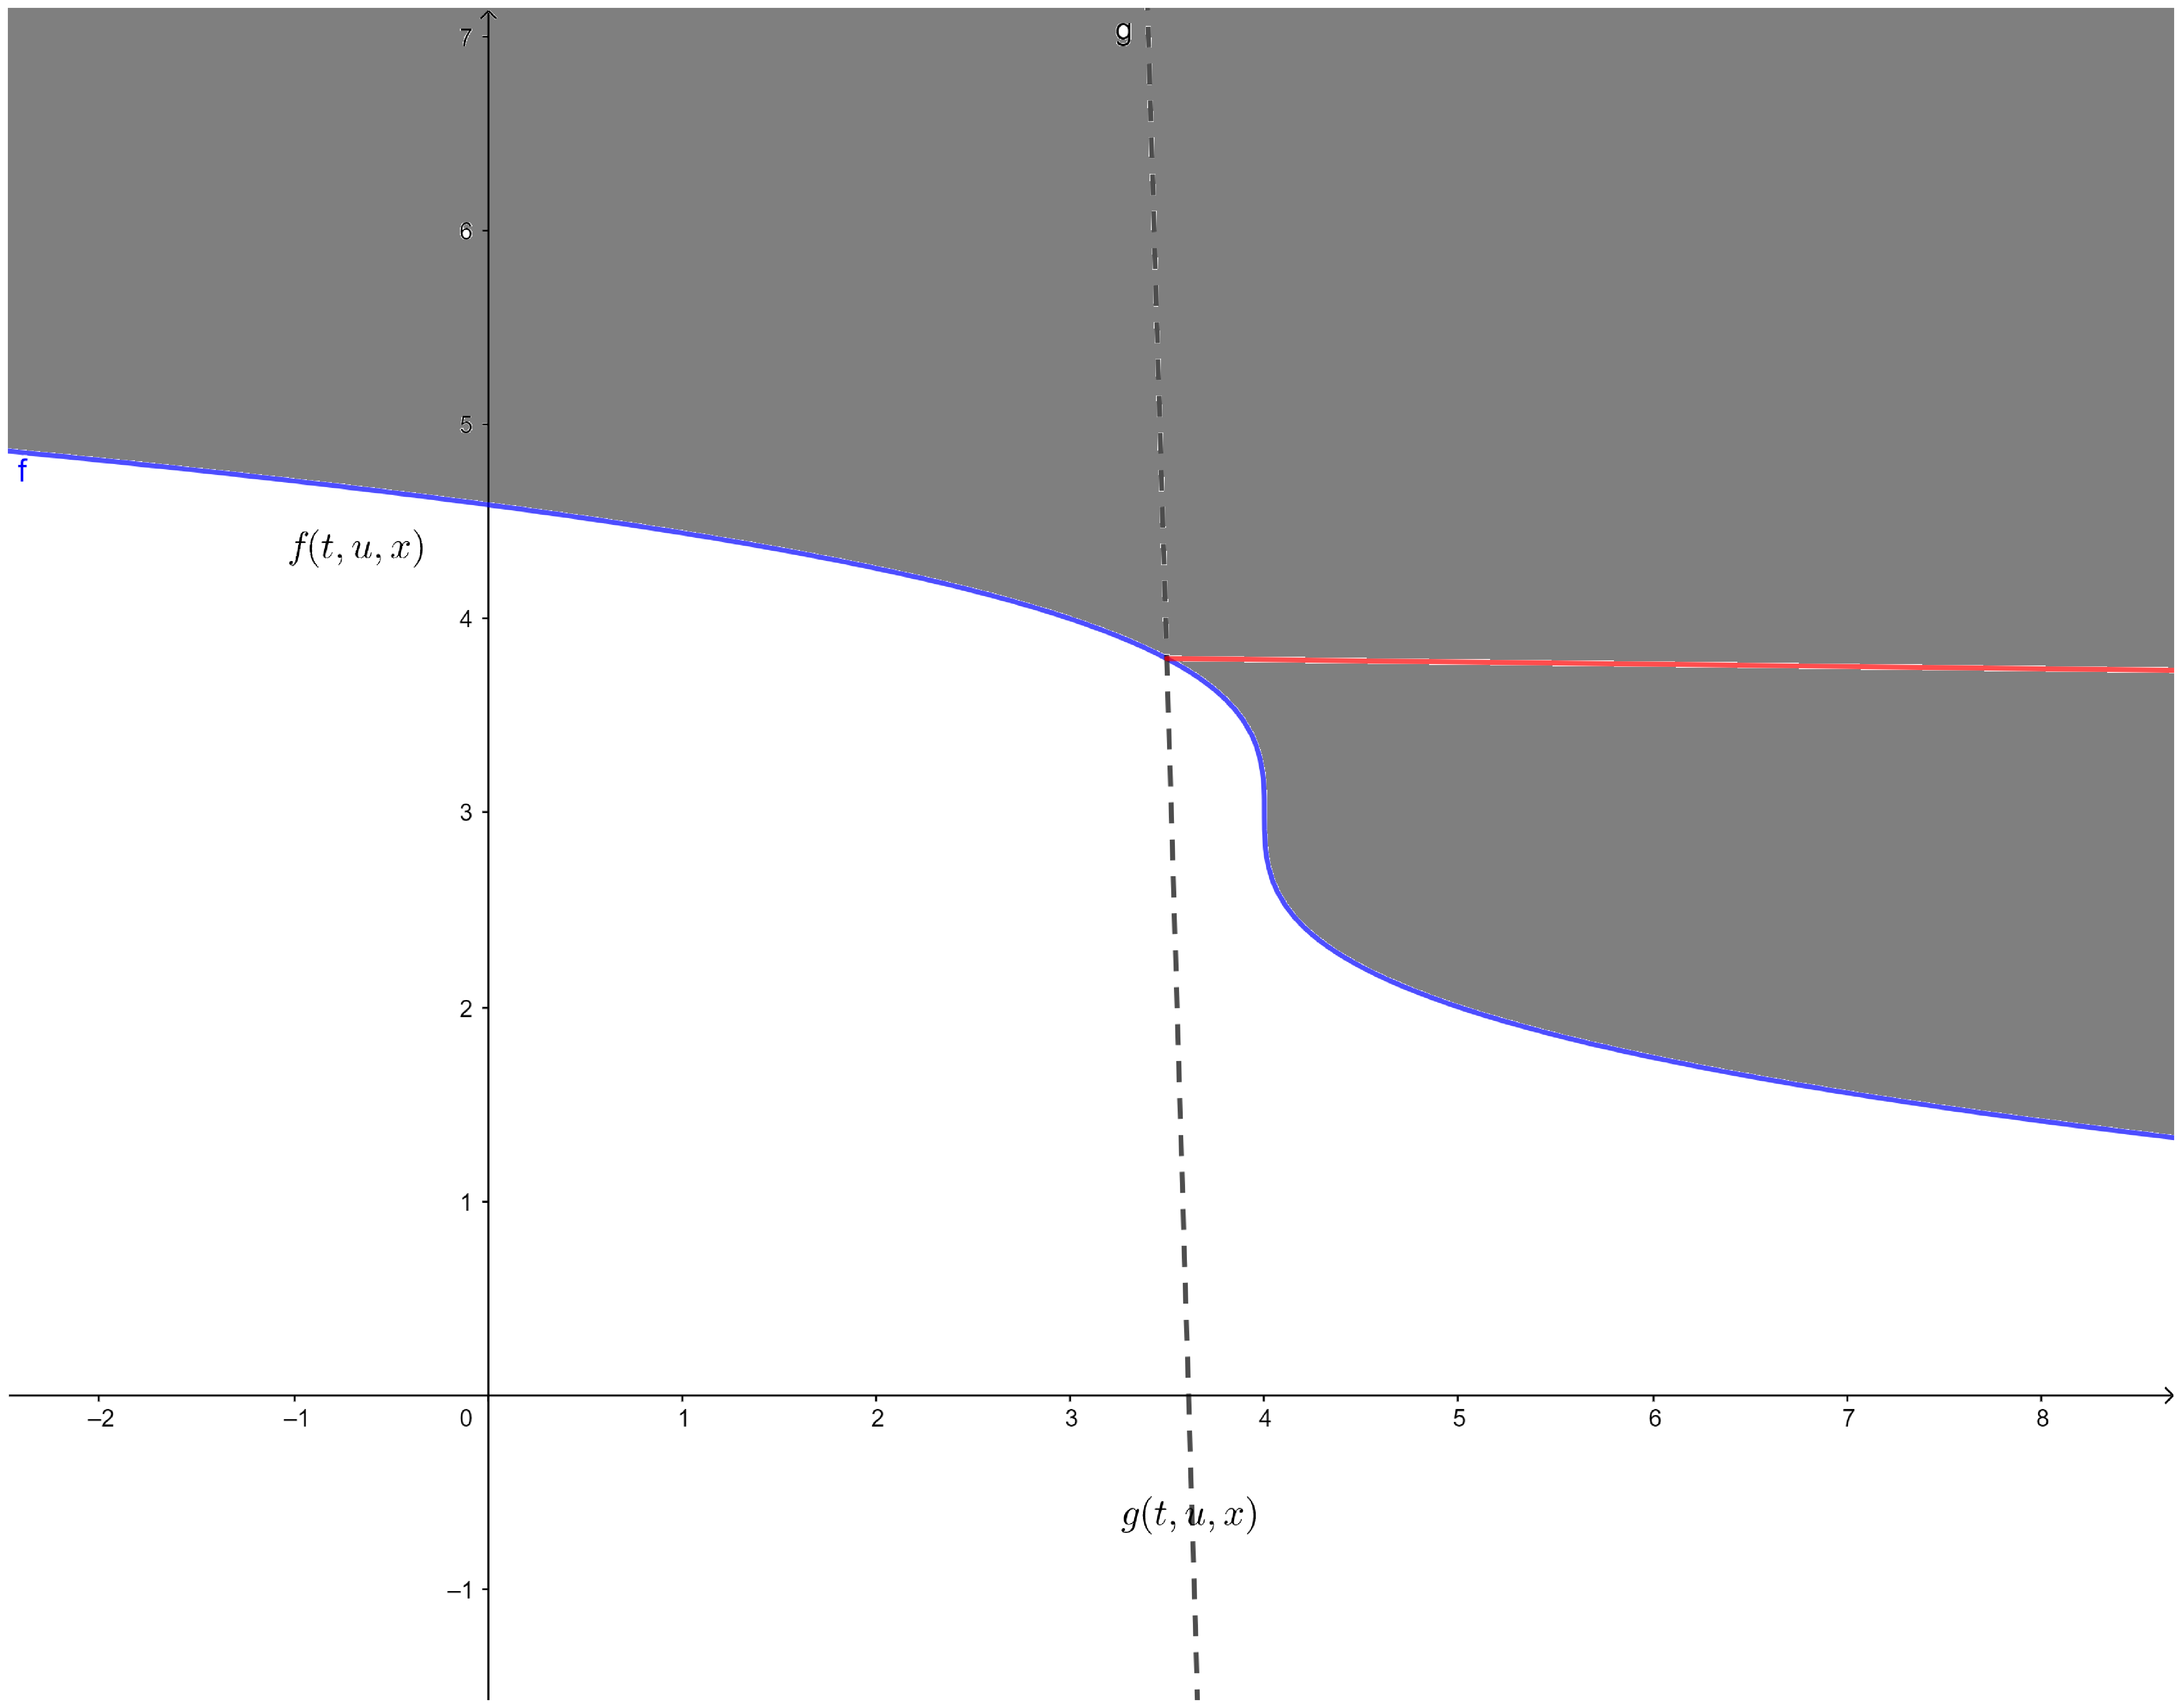
\includegraphics[width=\linewidth]{Feathergraphics/Conjunto_E.eps}
		\end{textblock*}
	}
\end{frame}
%%%%%%%%%%%%%%%%%%%%%%%%%%%%%%%%%%%%%%%%%%%%%%%%%%%%%%%%%%%%%%%%%%%%%%%%%%%%%%%%

\begin{frame}[plain]
	\begin{textblock*}{60mm}(5mm,5mm)
		\begin{graybox}{Hypothesis:}
			\begin{enumerate}[(\textbf{{C}}-1)]
				\item
					$
					f:\mathbb{R}_{+}\times U
					\times \mathbb{R}^n\rightarrow 
					\mathbb{R}^n
					$ is measurable, satisfies a lipchitz
					condition in $x$,
					$
					|f(t,u,0)|\leq L,\,
					\forall\,(t,u)\in
					\mathbb{R}_{+}\times U .
					$
				\item
					$
					g:\mathbb{R}_{+}\times U\times 
					\mathbb{R}^n\rightarrow \mathbb{R},
					$ 
					$
					h:\mathbb{R}^n\rightarrow \mathbb{R}
					$ are measurable, and
					\begin{align*}
					&|g(s,u,x_1)-g(s,u,x_2)|+\\
					&|h(x_1)-h(x_2)|\\
					&\leq \omega(|x_1|\vee |x_2|,|x_1-x_2|)
					\end{align*}
					$
					\forall\, (s,u)\in \mathbb{R}_{+}
					\times U,x_1,x_2\in \mathbb{R}^n
					$.
				\item
					For a.a. $t\in[0,T]$, Cesari property holds $\forall$ $x\in \mathbb{R}^n$.
			\end{enumerate}	
		\end{graybox}
	\end{textblock*}


	
	\begin{textblock*}{55mm}(70mm,15mm)
		\begin{graybox}{Existence Theorem}
			Let ($\mathbf{C}$-1)-($\mathbf{C}$-3) hold. Then problem $(OC)$ admits at least one optimal pair.
		\end{graybox}
	\end{textblock*}
\end{frame}

%%%%%%%%%%%%%%%%%%%%%%%%%%%%%%%%%%%%%%%%%%%%%%%%%%%%%%%%%%%%%%%%%%%%%%%%%%%%%%%%
